As we see in \cite{dreyer2009}, modeling attempts that describe how infectious diseases spread can be traced back to Bernoulli in 1760 in smallpox studies. Nowadays, based on dynamic systems models, these are still being analyzed. However, another interesting way to address such a problem is to note that diseases are spread through social networks, which can be very well represented by graphs.
Another problem very close to that of spreading diseases is the spreading of opinions in social networks, as well as of faults in computer networks. These have ample literature, as we can see in some of the early articles in these areas: \cite{poljak1983}, \cite{degroot1974} and \cite{french1956}.

According to \cite{dreyer2009}, the problem of irreversible conversion processes is defined as a model where given a $ G = (V, E) $, $ V $ being the set of vertices and $ E $ the set of edges, and each vertex $ v_{i}$ is in a state $ x_{i} ={0, 1}$ at a given time instant $ t $. The process is said irreversible because when a vertex enters the $ 1 $ state, or also said "infected", it will remain infected in the rest of the process.
The goal of this paper, however, is to characterize irreversible processes, where, in addition to being irreversible, each vertex assumes state 1 from state 0 if at least $ k $ of its neighbors are already infected. To find the smallest set of vertices, called the irreversible conversion set k, in which all the vertices of this set are infected at the beginning of the process, and in the end, will lead to the infection of all the vertices of the graph, shown to be an NP- complete for any $ k $ greater than 2. In sequence, \cite{chen2009} show the NP-completeness of the problem for $ k = 2 $, responding to the open conjecture proposed by \citeauthor{dreyer2009}.

In addition to proving the conjecture, \citeauthor{centeno2011} also show results for a generalization of the above-mentioned problem. In this more general form of the problem, the number of infected neighbors required for vertex infection is modeled by any function $ f: V \rightarrow \mathbb{Z} +$, instead of the previously used constant $ k $ , being denoted by $ irr_{f} (G) $. The results obtained in this paper describe a general reduction principle for $ irr_{f} (G) $, which leads to efficient algorithms for graphs with simple structure blocks, such as trees and chordal graphs.

In the article \cite{chopin2014}, the problem is called \textit{Target Set Selection}, and we see that in addition to generalizing the irreversible conversion set k, $ irr_{f} $ generalizes others problems in well-known graphs, such as Dominating Set with thresholds in \cite{Cordasco2018}, Vector Dominating Set in \cite{Cicalese2013}, K-Tuple Dominating Set \cite{Liao2003}, Vertex Cover, where the threshold function describes the degree value of each vertex and proved in \cite{chen2009}, r-Neighbor Bootstrap Percolation in \cite{balogh2009}, and dynamic monopolies in \cite{Khoshkhah2012}.

In \cite{Reddy2010} we see that for the class of bipartite graphs, the problem is NP-complete, but for the tree classes,
clicks, complete split graphs, threshold graphs and chain graphs, polynomial algorithms were found. Also studied as Target Set Selection, this problem is shown in \cite{BenZwi2009} to be $n^{\mathcal{O}(w)}$ with $n$ and $w$ being respectively the number of vertices and the graph's\textit{ treewidth}, which roughly measures the degree in which a given graph is similar to a tree in a very deep structural sense. This helps us to see how this problem will probably behave in instances where the graph is farther from a tree.

\citeauthor{Ackerman2010} also show a few extra bownds for this problem. Their upper bound implies that there are always Perfect Target Sets, the minimun set of initial infected vertices that infects the whole graph,  of size at most $|V|/2 $ and $ 2|V|/3$ under majority  $f(v)=\lceil deg_{in}(v)/2 \rceil $ and strict majority $f(v)=\lceil (deg_{in}(v) + 1)/2 \rceil$ thresholds . They also define a combinatorial model for the Target Set Selection problem relying on the idea that finding a way of directing the graph edges forming a directed acyclic graph, similarly to the way the infection spreads throw out the graph, respecting the rule where the infection only spreads if the vertex has sufficient edges pointing to it.  Unfortunately, this paper does not present experimental results for this model, making it difficult to compare our model to it. 

When we look for works in the experimental area of irreversible conversion processes, we realize that these are very scarce in the literature.\citeauthor{amaral2015} uses genetic algorithms to find results for the minimal convergent set problem seen here and, in \cite{Soltani2019}, we have a model based on \citeauthor{Ackerman2010}'s model,  where both are compared in the paper's experimental results. We will compare our model against \citeauthor{Soltani2019} models, since the code and instances are more easily accessible, and seem to show concrete results against the already well stablished model presented by \citeauthor{Ackerman2010}.


The version of the problem with the threshold function $ f (v, t) $ that changes over time and adds a maximum time-out for the total infection of the graph is seen in \cite{rautenbach2014}. In this article, we see that if G is a forest or a click, \citeauthor{rautenbach2014} presents efficient algorithms that compute $ irr (G, t_d, f) $. In addition, upper and lower bounds are tested based on counting and probabilistic arguments. For the special choices of $ t_d $ and $ f $, the parameter $ irr (G, t_d, f) $ coincides with well-known graph parameters related to the dominance and independence of the graph.

When considering the problem of spreading an infection in a square grid where the infection spreads to an uninfected grid square if at least two of the neighboring squares are infected, \citeauthor{centeno2010} show that this problem can be seen in a context of convexity of graphs. Given a $ G $ graph and a $ C $ collection of subsets of the vertex set $ V (G) $ of $ G $, the pair $ (G, C) $ is a convexity of the graph if $ \emptyset \in C $, $ V (G) \in C $ and $ C $ is closed under intersection.


Several natural convexities of graphs are defined in terms of paths. If $ \mathcal{P} $ is a set of paths in some graph $ G $ and $ C $ is the collection of all subsets $ C $ of $ V (G) $ so that, for each path $ P $ in $ \mathcal{P} $ between two vertices in $ C $, set C contains all vertices of $ P $, so $ (G, C) $ is a convexity of the graph. To capture the scattering process in the aforementioned grid, $ P_3 $ is chosen as the set of all order paths 3 in some $ G $ graph. Specifically, we call a set $ C $ of vertices in a graph $ G $ of $ P_3 $ - convex if, for each path $ uvw $ in $ G $ with $ u, w \in C $, $ v $ belongs to $ C $. Or, in other words, $ C $ is $ P_3 $ -convex in $ G $ if and only if no vertex in $ V (G) \setminus C $ has at least 2 neighbors in $ C $. This problem is similar to ours where the threshold function is constant equal to $2$. In \cite{centeno2010}, among other results, we see that for a given graph $ G $ and an integer $ p $, assert whether the set of vertices of $ G $ can be partitioned into $ p $ sets $ P_3 $ - convex not empty is NP-complete. \cite{lacerda2017} formulates integer models for this problem and presents experimental results regarding this instance of our problem.

\citeauthor{dreyer2009} also propose another problem in the context of irreversible conversion processes, this involving vaccinating vertices of a graph. Thus, a vertex that does not have the characteristic / disease can be vaccinated, which prevents it from being infected in the future. The objective is to find the least (or better) set of vertices, in order to prevent the feature from reaching a certain subset of the vertices. The number of vaccines may also be limited, and the question is as many vertices as possible to be protected with the available resources.

Figure \ref{fig:graph2} 
shows some of the main graph classes, with some of the theoretical results obtained so far for the minimum convergent set problem. These are presented by an inclusion graph, where if two classes are neighbors and $\overrightarrow{class_1 class_2}$, then $class_1 \supset class_2$.

\begin{figure}
  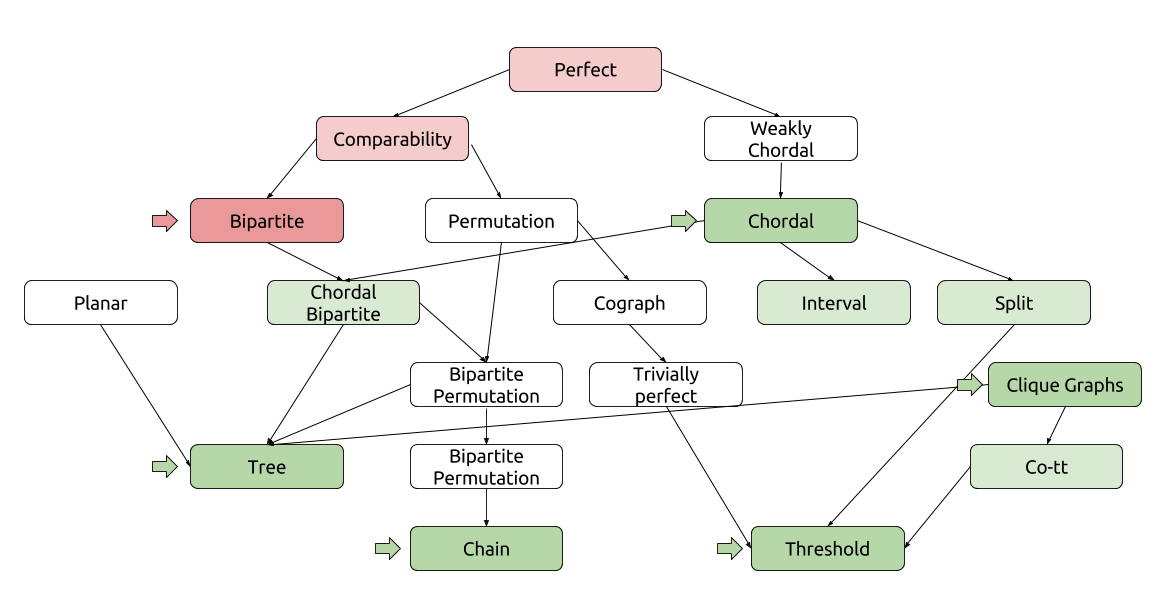
\includegraphics[width=18cm,center]{img/Figure2-1.png}
  \caption{
  Graph class inclusion graph: In red, classes proven NP-complete for the problem; In green, classes with polynomial algorithms. In red and light green, classes that are contained / contain other classes, consequently have the same results. Open classes are blank, with no definite result as to their complexity.}
  \label{fig:graph2}
\end{figure}

Or, for clarity on the results shown in the previous figure, see Table \ref{tab:2} with the theoretical results of some classes of graphs, and the reference to the test article:
\begin{table}[!htbp]
\caption{Resultados do problema para algumas classes de grafos e suas referências} \label{tab:2}
\begin{center}
 \begin{tabular}{||c c c||} 
 \hline
 Classe & Complexidade & Referência \\ [0.5ex] 
 \hline\hline
 Árvores & Polinomial & \cite{centeno2011} \\ 
 \hline
 Cordal & Polinomial & \cite{centeno2011} \\ 
 \hline
 Bipartido & NP-completo & \cite{Reddy2010} \\
 \hline
 \textit{Chain} & Polinomial &  \cite{Reddy2010}  \\
 \hline
 \textit{Threshold} & Polinomial & \cite{chen2009}\\
 \hline
 Clique & Polinomial & \cite{Nichterlein2013} \\
 \hline
\end{tabular}
\end{center}
\end{table}

As we can see, these results show how the treewidth strongly defines the difficulty of our problem.  


%Convex hull for P3  https://www.sciencedirect.com/science/article/pii/S1571065313002333
% parametrized stuff
%  * http://www.akt.tu-berlin.de/fileadmin/fg34/publications-akt/tss-long.pdf
%  * https://arxiv.org/pdf/1610.07530.pdf

% model with no results: https://link.springer.com/content/pdf/10.1007/s10878-018-0256-z.pdf
%model to maximize number of infected at the end: http://journals.tubitak.gov.tr/elektrik/issues/elk-18-26-6/elk-26-6-46-1802-212.pdf

% paper to beat. Has instances and concrete model. https://link.springer.com/content/pdf/10.1007/s10479-018-3107-5.pdf \cite{Soltani2019}

% M campelo work https://sol.sbc.org.br/index.php/etc/article/view/3176/3138

%Solução grande??????? Pedir vinicius  https://www.sciencedirect.com/science/article/pii/S1571065313002485#!